\ifgerman{\chapter{Zukunftige Arbeiten}}{\chapter{Future Work}}
\label{futurework}

In this section, we describe ways to improve the visualization techniques presented in this work. The general feedback shown in  \hyperref[sec:4.6]{Section 4.6} forms as a base for our future work.
We describe the most important feedback and provide mockups for each of them.


\begin{myindentpar}{0cm}
\textbf{Ratio plot with positive and negative influences}: The Ratio plot does not distinguish between positive and negative influences of configuration options. Hence, 33\% of the interviewees suggested to improve the ratio plot by having an axis separating configuration options and interactions that indicate positive and negative influence. \hyperref[posNegBefore]{Figure 7.1}, presents the current state of the ratio plot and \hyperref[posNegAfter]{Figure 7.2}, presents the mockup of the ratio plot with the positive and negative influences. 

\begin{figure}[ht]
\centering
\label{posNegBefore}
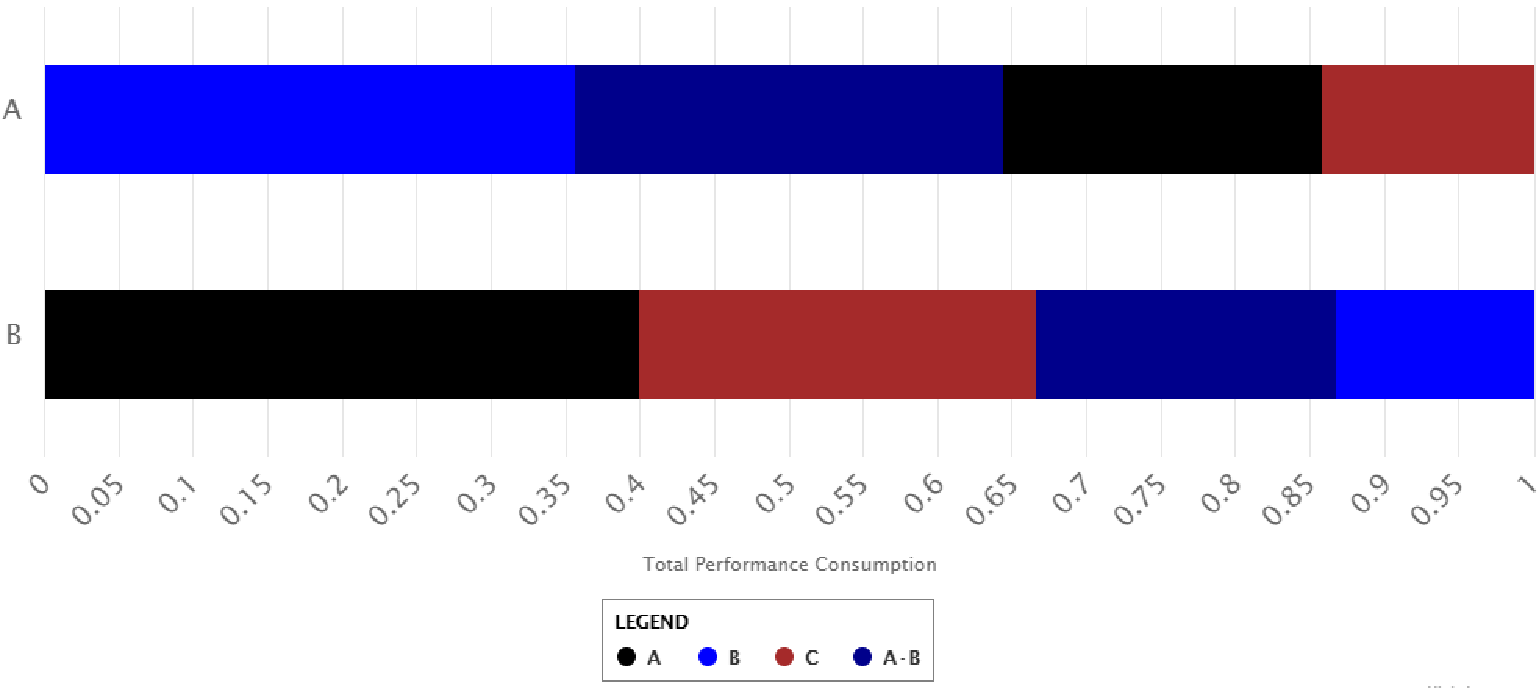
\includegraphics[width=15cm,height=15cm,keepaspectratio,]{pics/ratio_plot_positvie_negative_before.pdf}
\caption[Current state of the ratio plot]{Mockup of the ratio plot with configuration options A and B and interaction \mbox{A $\cdot$ B} of 2 performance-influence models A and B}
\end{figure}

\begin{figure}[ht]
\centering
\label{posNegAfter}
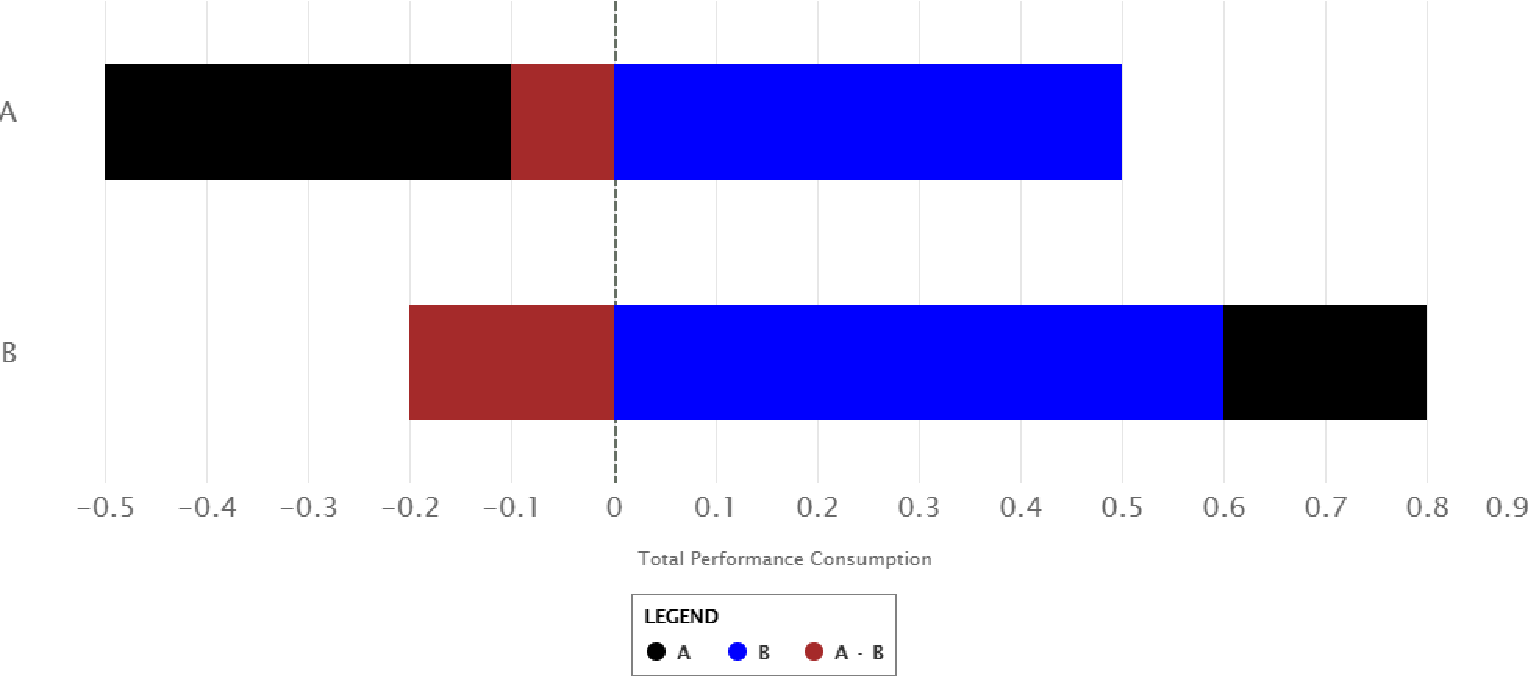
\includegraphics[width=15cm,height=15cm,keepaspectratio,]{pics/ratio_plot_positvie_negative_after.pdf}
\caption[Ratio plot with axis between positive and negative influences]{Mockup of the ratio plot with configuration options A and B and interaction \mbox{A $\cdot$ B} of 2 performance-influence models A and B. For performance-influence model A, the interaction \mbox{A $\cdot$ B} and configuration option A are on left side on the axis and configuration option B is on the right side of the axis, indicating negative and positive influences respectively. Similarly, for performance-influence model B, the interaction \mbox{A $\cdot$ B} is on the left side of the axis and configuration options A and B are on the right side of the axis }
\end{figure}


\textbf{Ratio plot without sorting functionality}:  Another improvement on the ratio plot would be to show all configuration options and interactions in the same order for all performance-influence models. Currently, we display the configuration options and interactions in a sorted order from highest to lowest relative performance influence for each performance-influence model. However, sorting the configuration options and interactions makes the comparison between performance-influence models more difficult.  \hyperref[sameOrderAfter]{Figure 7.3},  presents the mockup of the ratio plot with the feature and  \hyperref[posNegBefore]{Figure 7.2}, presents the current state of the ratio plot.

\begin{figure}[ht]
\centering
\label{sameOrderAfter}
 %- \textbf{Your title}\par\medskip
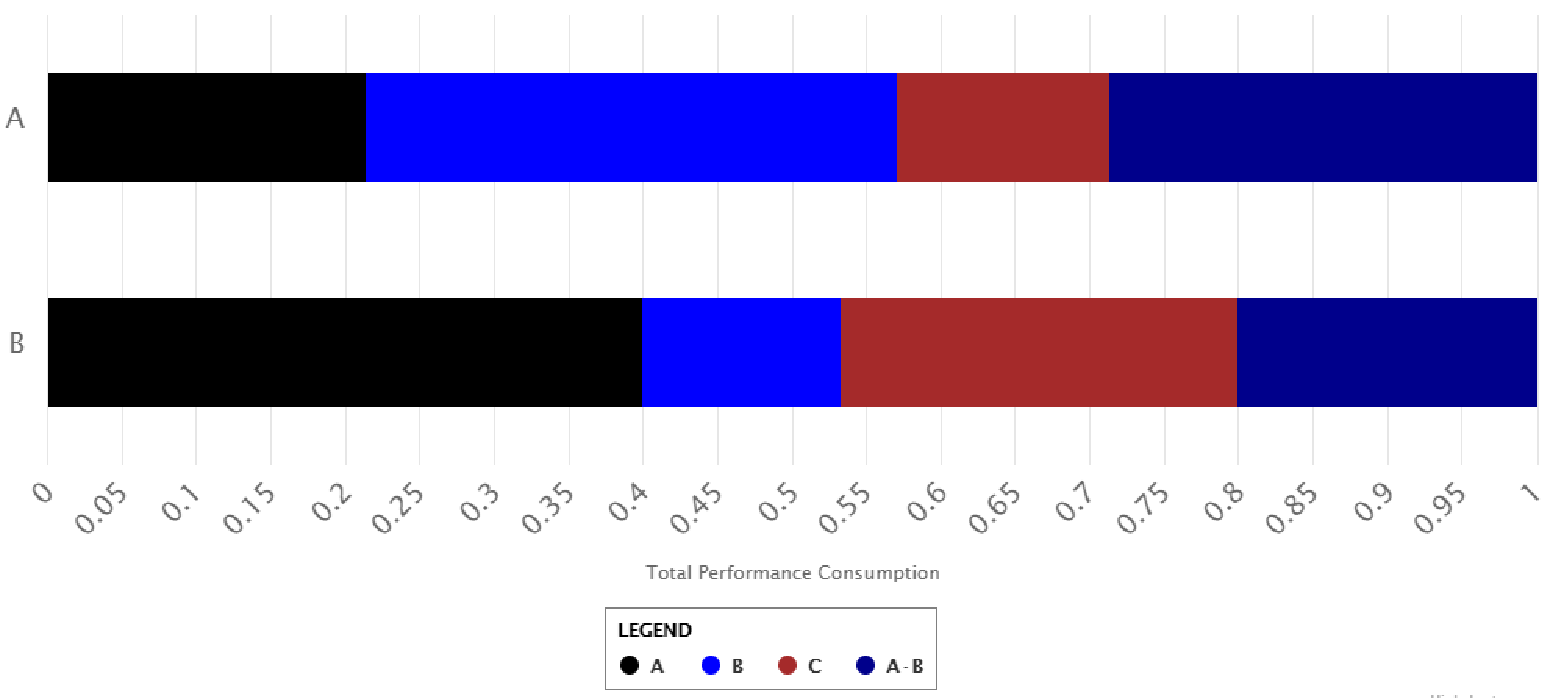
\includegraphics[width=15cm,height=15cm,keepaspectratio,]{pics/ratio_plot_without_sorted_order_after.pdf}
\caption[Ratio plot without sort functionality]{Mockup of the ratio plot with configuration options A and B and interaction \mbox{A $\cdot$ B} of 5 performance-influence models all displayed in the same order}
\end{figure}

\textbf{Sorting Feature}: An improvement suggested for the radar and the text plot was to present the configuration options and interactions in an order from highest to lowest relative performance influence. This would help the users perception in finding the most relevant configuration option or interaction easily. \hyperref[relevanceBefore]{Figure 7.4}, presents the current state of the radar plot and \hyperref[relevanceAfter]{Figure 7.5}, is a mockup of the revised the radar plot.

\begin{figure}[H]
\centering
\begin{adjustbox}{width=1\textwidth}
\begin{minipage}[8cm]{.44\textwidth}
 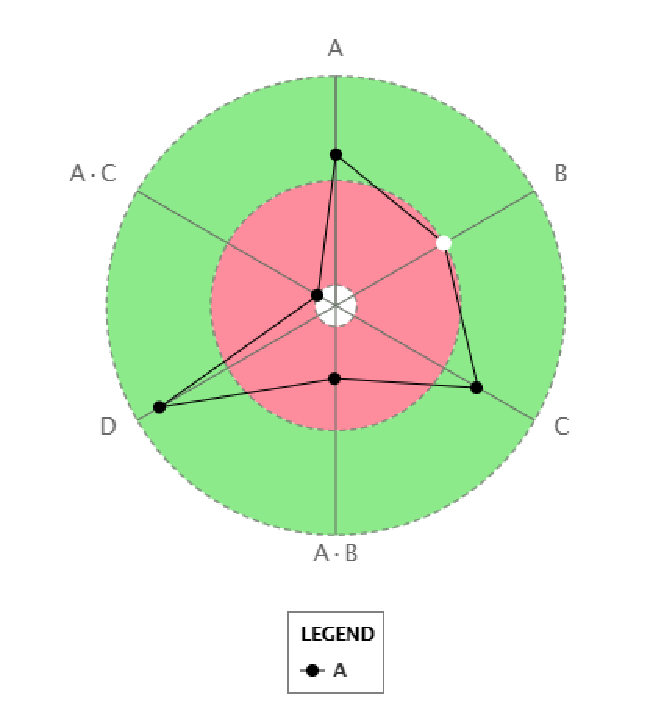
\includegraphics[width=7cm,height=7cm,keepaspectratio,]{pics/sorted_order_before_radar.pdf}
\caption[Radar plot without sorting feature]{Radar plot with configuration options and interactions displayed without a definite order.}\label{relevanceBefore}
\vspace{\baselineskip}
\end{minipage}
\begin{minipage}[8cm]{.44\textwidth}
 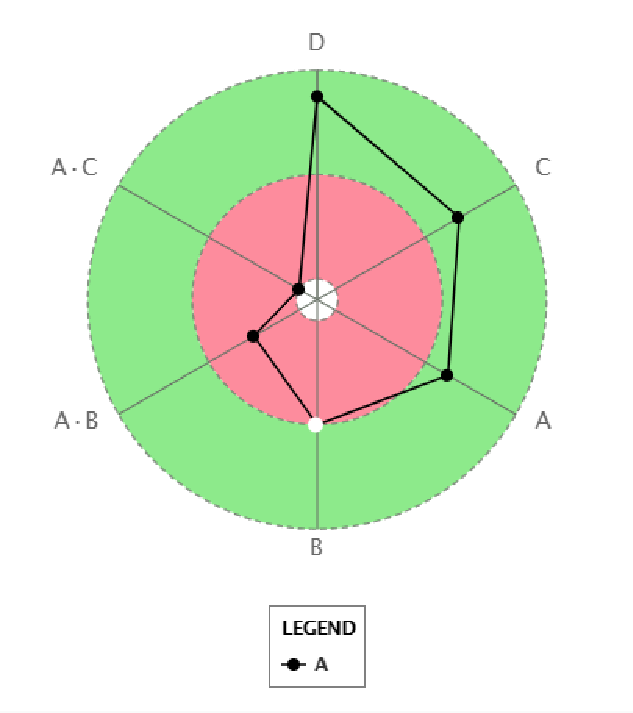
\includegraphics[width=7cm,height=7cm,keepaspectratio,]{pics/sorted_order_after_radar.pdf}
\caption[Radar plot with sorting feature]{Radar plot with configuration options and interactions sorted according to the relative performance influence they contribute.} 
\label{relevanceAfter}
\vspace{\baselineskip}
\end{minipage}
\end{adjustbox}
\end{figure}

\end{myindentpar}
